\subsection {Energiespeicherung und Verhalten von Solarzellen}      % 2.4
    \subsubsection{Theoretische Betrachtung}                            % 2.4 a
        \textbf{Diskussion}
        \newline
        \par Ein Kondensator besteht aus zwei Metallflächen, die durch einen Isolator getrennt sind. Er dient zur Ladungsspeicherung, indem man ihn an eine Spannungsquelle schaltet. Die davor gleichmäßig verteilten Elektronen werden vom Minus-Pol gezogen, welches mit dem Plus-Pol der Quelle verbunden ist. Somit wird der Kondensator elektrisch geladen. Würde man jetzt die Spannungsquelle mit einem Widerstand wechseln, dann würde der Kondensator als Spannungsquelle fungieren und sich entladen. Der Minus-Pol des Kondensators, wo sich früher die Elektronen gelagert haben wird neutral, indem die Elektronen über dem Widerstand vom Plus-Pol weggezogen werden. Der Isolator sorgt dafür, dass der Minus- und Plus-Pol nie direkt in Verbindung kommen, so dass die Elektronen immer über einen Leiter wandern müssen.
        
        $$
            \tau = R * C = 500 \Omega * 220mF = 110s
        $$
        
    \subsubsection{Messung}                                             % 2.4 b
        \textbf{Methode/Materialien}
        \newline
        \par Hier soll an der bisherigen Schaltung ein Speicherkondensator (V =5,5 V; C =220,0 mF) angeschlossen
        werden. Unter konstanter Bestrahlung der Solarzelle wird die Spannung beim Aufladen des
        Kondensators gemessen. Als nächstes soll das Licht ausgeschaltet werden und der Kondensator soll mit
        einem 500 Ohm Widerstand angeschlossen werden, damit er sich entlädt.
        \vspace{4mm}
        \newline
        \textbf{Ergebnis}
        \newline
        \par
        \begin{figure}[H]
            %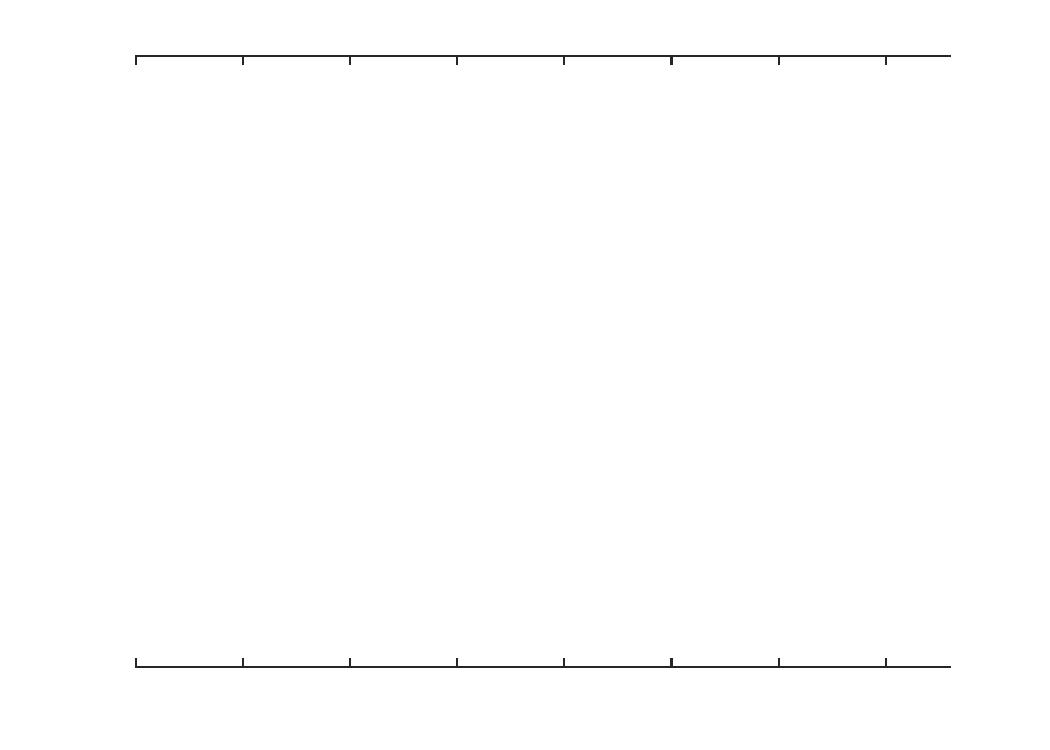
\includegraphics{leistung_langzeit}
            \def\svgwidth{\textwidth}
            \input{spannung_aufladen.pdf_tex}
            
            \caption{Spannungsverlauf bei Aufladen des Kondensators}
        \end{figure}
        \begin{figure}[H]
            %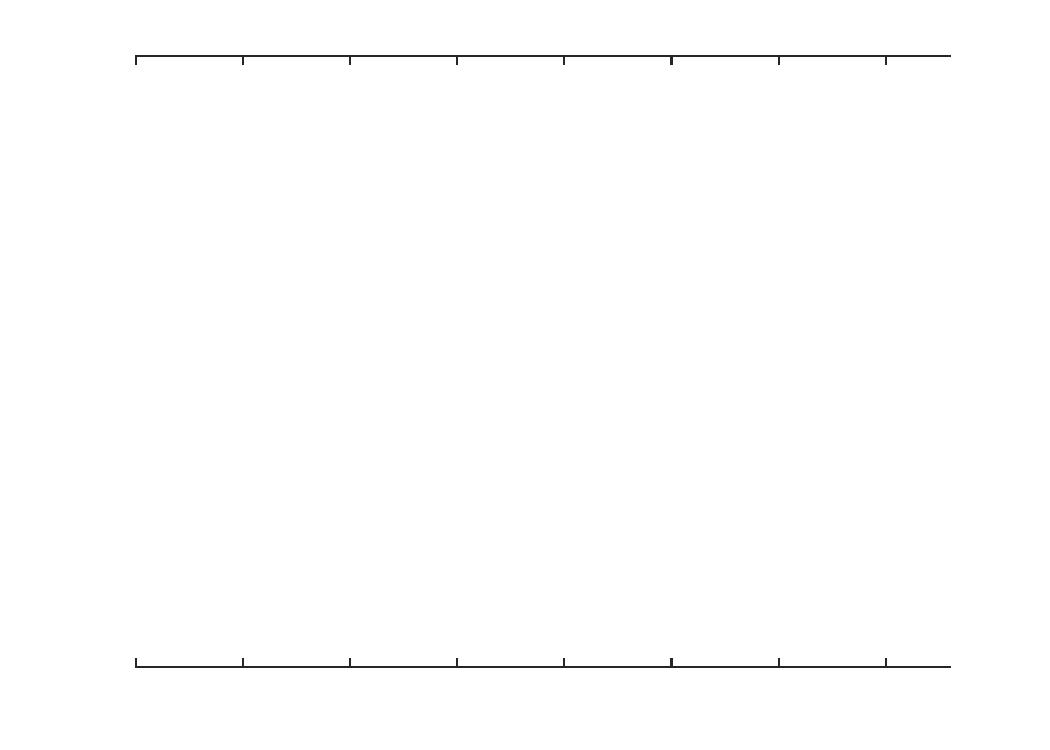
\includegraphics{leistung_langzeit}
            \def\svgwidth{\textwidth}
            \input{spannung_entladen.pdf_tex}
            
            \caption{Spannungsverlauf bei Entladen des Kondensators}
        \end{figure}
        
        \clearpage
    \subsubsection{Modellbildung}                                       % 2.4 c
        \textbf{Diskussion}
        \newline
        \par Die in der letzten Teilaufgabe gezeigten U-I-Diagramme sind hier zu vergleichen. Beim Aufladen sieht
        man, dass je größer die Spannung wird, umso mehr sich die Stromstärke den Wert Null annähert. Die
        Kurve fängt bei einem Wert von ungefähr 2.7mA an, wo noch fast keine Spannung fließt. Die
        Stromstärke sinkt rapide. Je näher sie sich der Null nähert, umso langsamer sinkt sie. Die Spannung
        dagegen steigt kontinuierlich, bis sie ihren Grenzwert bei ungefähr 0.42V erreicht. Beim Entladen sollte
        man den Graphen von rechts nach links lesen, weil die Spannung sinkt. Die Kurve fängt bei ca. -3.5mA
        und 0.36V an. Hier sind die Werte von der Stromstärke im negativen Bereich zu sehen. Wieder nähert
        sich die Stromstärke der Null an, aber diesmal indem sie steigt. Je kleiner die Spannung ist, umso größer
        wird die Stromstärke.
        \par Beim Aufladen eines Kondensators, steigt die Spannung bis zum Maximalwert. Dabei steigt auch der
        Widerstand des Kondensators, denn er kann ab einer bestimmten Spannung zerstört werden. Weil es
        weniger Elektronen gibt, die auf dem Pluspol des Kondensators sind, fließt weniger Strom durch. Wird
        der Maximalwert der Spannung erreicht, dann fließt kein Strom mehr. Der Widerstand des
        Kondensators wird dabei unendlich groß.
        \par Beim Entladevorgang wirkt der Kondensator wie eine Spannungsquelle mit einem sehr kleinen
        Innenwiderstand. Es fließt ein Strom in der entgegengesetzten Richtung, was erklärt, warum die
        Stromstärke im negativen Bereich liegt. Die Spannung sinkt vom Maximalwert auf Null und genauso
        sinkt die Stromstärke. Wenn der Kondensator entladen ist, dann fließt kein Strom mehr.
        Um die Solarzelle besser zu beschreiben, soll eine Stromquelle als Modell benutzt werden, denn die
        Stromstärke verändert sich im Verhältnis zur Spannung kaum.

        \clearpage
    \subsubsection{Gesamtenergie und Wirkungsgrad}                      % 2.4 d
        \textbf{Methode/Materialien}
        \newline
        \par
        \begin{figure}[H]
            \lstinputlisting[language=Matlab, frame=single, firstline=17]{messungen/Aufgabe_2_4/Energie.m}
            \caption{Matlab-Skrip zur Berechnung des Wirkungsgrades}
        \end{figure}
        \vspace{4mm}
        %\newline
        \textbf{Ergebnis}
        \newline
        \par Wirkungsgrad: 79.42\%
        \vspace{4mm}
        \newline
        \textbf{Diskussion}
        \newline
        \par Recherchen zeigen (Quelle aus Internet), dass der Wirkungsgrad unserer Messung um 10 % abweicht, da
        sie bei 90% liegen sollte. Diese Differenz kann auf mehrere Faktoren zurückgeführt werden.
        In der letzten Teilaufgabe ist zu sehen, dass das Aufladen des Kondensators bei ca. 0.42V aufhört und
        das Entladen bei ca. 0.36V anfängt. Dies bedeutet, dass zwischen den beiden Vorgängen Spannung
        verloren gegangen ist. (Speicherdauer)
        \par Außerdem könnten es Messfehler geben. Z.B. könnte der Raum beim Entladevorgang nicht dunkel
        genug gewesen sein, sodass die falschen Spannungen gemessen wurden. Darüberhinaus ist zu beachten,
        dass die Wärmeverluste immer mitgemessen wurden.
